% English version of relatorio.tex: same content, results and figures (fig-*-en.pdf).
% Build: latexmk -pdf report.tex

\documentclass[11pt,a4paper]{article}

\usepackage[T1]{fontenc}
\usepackage[utf8]{inputenc}
\usepackage[english]{babel}
\usepackage{lmodern}
\usepackage{microtype}
\usepackage[margin=2.5cm]{geometry}
\usepackage{amsmath}
\usepackage{graphicx}
\usepackage{array}
\usepackage{booktabs}
\usepackage[font=small,labelfont=bf]{caption}
\usepackage[round]{natbib}
\usepackage{xurl}
\usepackage[hidelinks]{hyperref}

\setlength{\parskip}{0.3em}

\newcommand{\note}[1]{\par\vspace{0.3em}{\footnotesize\raggedright #1\par}}

\title{High-Impedance Fault Region Locator \\ as Firmware on a Simulated Microcontroller}
\author{Pedro Henrique Faluba Martins \\[0.3em]
  \small Universidade Federal de Minas Gerais (UFMG), School of Engineering \\
  \small Undergraduate Program in Electrical Engineering \\[0.3em]
  \small Technical report}
\date{Belo Horizonte, 2026}

\hypersetup{pdftitle={High-Impedance Fault Region Locator as Firmware on a Simulated Microcontroller},
            pdfauthor={Pedro Henrique Faluba Martins}}

\begin{document}

\maketitle

\begin{abstract}
\noindent
A previous work selected fifteen features, built on the discrete Fourier, Stockwell and wavelet transforms of substation measurements, for locating the region of a high-impedance fault, and argued that they are cheap to compute. This report tests that argument on an embedded target. The complete locator, feature extraction followed by a classifier, was implemented as C firmware for an ARM Cortex-M4F microcontroller (STM32F407) simulated in Renode, verified against a Python reference, and measured in flash, RAM, stack and executed instructions across 80 configurations of feature set, model, model complexity and compiler optimization. The cost lies in the feature extraction, 17.17 million instructions per window, 60\% of it in the wavelet transform, while inference takes at most 0.02\% of the total. The selected set needs 4.4 times fewer instructions than all 7056 candidate features without losing accuracy with a random forest (macro-F1 0.781), and outperforms every random set of the same size at comparable cost. Flash is set by the model and RAM by the extraction; storing the raw window is the main obstacle to a real device.
\end{abstract}

% ----------------------------------------------------------
\section{Introduction}

High-impedance faults (HIFs) occur when an energized conductor touches a material of very low conductivity. They draw low, random and non-linear currents, which makes them hard to detect and locate with conventional protection \citep{[3]}. A previous work \citep{martins_tcc_en} proposed a systematic feature selection procedure for locating the region of an HIF from substation measurements alone. Its result was a set of fifteen feature families, extracted with the discrete Fourier, Stockwell and wavelet transforms over a 20-cycle window, which clearly outperformed random sets of the same size under nested cross-validation.

That work also argued that the selected features are cheap to compute, since extracting all 7056 features of one simulation took about 0.2\,s on a general-purpose processor, less than the duration of the window itself. The argument, however, was made on a personal computer, whereas protection and monitoring equipment in substations is typically embedded, built on microcontrollers with memory in the hundreds of kilobytes and no operating system. Running the locator on the measuring device itself would remove the communication with a control centre and its latency, but it is not known whether the transforms used, in particular the Stockwell and wavelet transforms, fit the resources of such a device, nor whether feature selection saves resources compared with using all candidate features.

Moreover, the previous work delivered a feature set rather than a trained model, leaving as future work an intelligent algorithm fed by that set. The choice of algorithm also matters on the device, since different model families take memory and processing in very different proportions.

The objective of this work is therefore to implement the complete locator, that is, the extraction of the selected features and a downstream classifier, as C firmware for a simulated ARM Cortex-M4F microcontroller, and to measure the memory and computation it needs in different configurations. To this end, the embedded implementation is first verified against the Python reference implementation; then the selected set, all candidate features, random subsets and the top features of the ranking are compared, combined with four model families, different model complexities and two compiler optimization levels.

% ----------------------------------------------------------
\section{Background}
\label{sec:background}
This section covers machine learning on microcontrollers and its tools, the platform adopted and its libraries, the functional simulation used to run it, and how works on HIF location with intelligent algorithms treat computational cost.

\subsection{Machine learning on microcontrollers}
Running machine learning models on microcontrollers, known as TinyML, means inference on devices with memory in the kilobytes and power in the milliwatts, without an operating system and without a mandatory link to servers \citep{warden_tinyml}. According to \citet{ray_tinyml}, the field is motivated by lower latency, lower energy use and less dependence on connectivity, at the price of severe memory and processing constraints that call for dedicated models and implementations.

The main tools are:
\begin{itemize}
    \item \textbf{TensorFlow Lite Micro:} an interpreter for neural networks trained in TensorFlow, aimed at microcontrollers and supporting 8-bit quantization, whose evaluation shows low resource use and small runtime overhead \citep{david_tflm}.
    \item \textbf{CMSIS-NN:} a library of neural network kernels optimized for Cortex-M processors, in 8- and 16-bit fixed point, reporting a 4.6-fold runtime gain over reference implementations \citep{lai_cmsisnn}.
    \item \textbf{emlearn:} a library that converts models trained in scikit-learn \citep{[52]}, such as decision trees, random forests and neural networks, into C code without dynamic memory allocation \citep{nordby_emlearn}. Because it covers classical machine learning models and not only neural networks, it is the tool adopted here.
\end{itemize}

For evaluation, MLPerf Tiny defines a standard set of tasks and metrics, namely accuracy, latency and energy, measured on real devices \citep{banbury_mlperf}. Its tasks, however, are keyword spotting, visual wake words, image classification and anomaly detection, where the model's input is the signal itself or a simple spectrogram. Problems like the one studied here, where feature extraction involves time-frequency transforms over several channels, are not represented.

\subsection{The Cortex-M4F platform and CMSIS-DSP}
Cortex-M4 processors implement the 32-bit Armv7E-M architecture, with a three-stage pipeline, signal processing instructions and an optional single-precision floating-point unit \citep{arm_cm4}. The STM32F407 microcontroller pairs this processor, with the floating-point unit, with 1\,MB of flash and 192\,KB of RAM, of which 64\,KB are core-coupled memory (CCM), accessible to the processor but not to the DMA controllers \citep{st_rm0090}. It is a widely used, low-cost microcontroller, which makes it representative of an embedded measuring device.

For signal processing, the CMSIS-DSP library provides routines optimized for the Cortex-M family, including the real fast Fourier transform (FFT) \citep{arm_cmsisdsp}. This transform, however, is only available for power-of-two lengths from 32 to 4096 points, a restriction that matters for the Stockwell transform, as discussed in Section~\ref{sec:method}.

\subsection{Functional simulation of microcontrollers}
Renode is a simulator that runs the binary compiled for the microcontroller unchanged, with models of each platform's peripherals, such as serial interfaces, and supports test automation through Robot Framework \citep{renode}. It counts the instructions the processor executes, but it is functional rather than cycle-accurate: it reproduces the program's behaviour without modelling the pipeline, flash wait states or instruction latencies. Instruction counts are therefore suitable for comparing configurations, but they do not correspond to execution time on a real device.

\subsection{Computational cost in HIF location}
The literature on HIF location based on intelligent algorithms relies mostly on artificial neural networks \citep{[5],[8],[28]}, as well as support vector machines \citep{[27]}, Gaussian process regression \citep{[25]} and comparisons between algorithms \citep{[2],[6]}, of which \citet{[6]} chooses an ensemble of decision trees. These works evaluate location performance, but treat the cost of running it qualitatively. \citet{[5]}, for example, highlight the simplicity and low implementation cost of their method, which uses substation measurements only, without quantifying the memory or processing it requires.

In the comparison made by \citet{martins_tcc_en}, the processing required by the region-oriented works is likewise described by the techniques used and the measurement points needed, and none of them reports memory or processing measurements on an embedded device. The previous work itself measured extraction time on a personal computer only.

Two observations frame the contribution of this work. First, TinyML tools and benchmarks focus on the model, whereas in HIF location the feature extraction involves time-frequency transforms potentially more expensive than the model itself. Second, HIF location works do not quantify the memory and processing needed on an embedded device. This work measures both, for the feature set obtained by \citet{martins_tcc_en}.

% ----------------------------------------------------------
\section{Method}
\label{sec:method}
This section describes the data, feature sets and models evaluated, the platform and the C implementation of the extraction, and then the procedures used to verify that the implementations agree, the measurement method and the configuration sweep. Figure~\ref{fig:pipeline} summarizes the method.

\begin{figure}[htb]
    \centering
    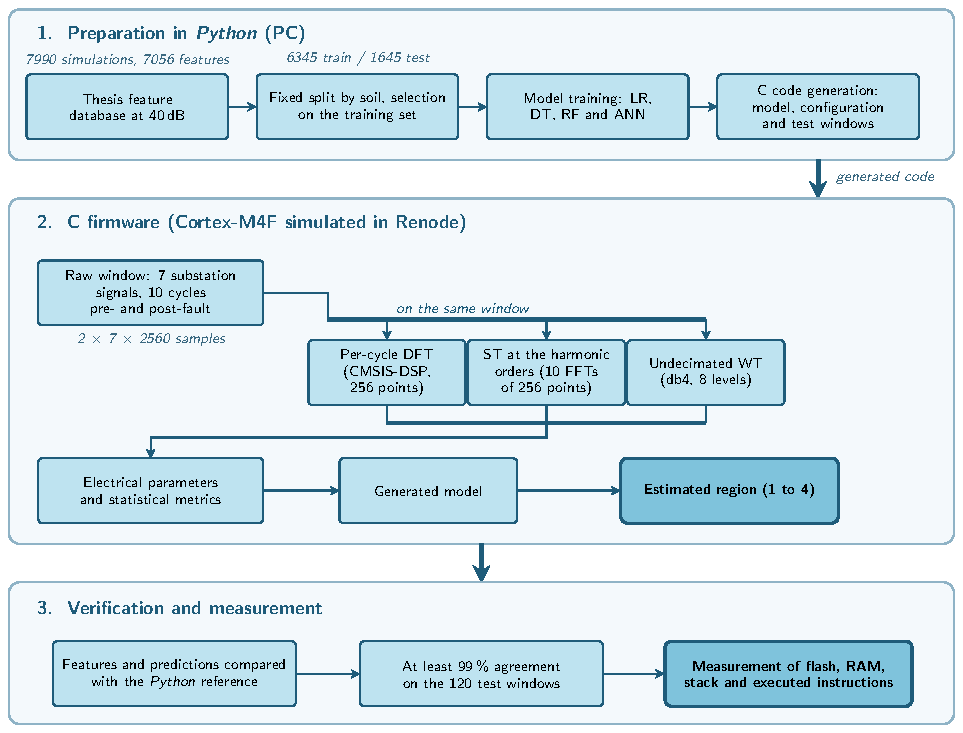
\includegraphics[width=\linewidth]{fig-pipeline-en.pdf}
    \caption{Implementation and evaluation flow of the locator as firmware.}
    \label{fig:pipeline}
\end{figure}

\subsection{Data and feature sets}
\label{sec:data}
The feature database built by \citet{martins_tcc_en} was used: 7056 features per simulation over 7990 HIF simulations on an adapted IEEE 34-node test feeder, at the 40\,dB noise level adopted in that work. The train/test split was fixed once and kept for every experiment. It holds out seven of the 34 HIF signals for testing, drawn with a fixed seed, which yields 6345 training and 1645 test simulations with the same proportion of regions. Splitting by HIF signal rather than by simulation keeps the same arc waveform from appearing in both training and test sets.

The ranking published by \citet{martins_tcc_en} was obtained on all simulations, including those that form this work's test set. For that reason, that work's selection chain, namely correlation clustering, filtering, an embedded stage, a wrapper stage and stability selection, was re-run unchanged on the training simulations only, over one hundred runs. The resulting stability index was 0.256, below the 0.315 obtained on the full set, as expected given the fewer HIF signals in each subsample, and the resulting set shares ten of its fifteen clusters with the published one. This set, shown in Table~\ref{tab:top15}, is the reference set of this work.

\begin{table}[htb]
  \centering
  \caption{Fifteen-feature set selected on the training simulations.}
  \label{tab:top15}
  \begin{tabular}{rllllll}
  \toprule
  \textbf{\#} & $\boldsymbol{\pi}$ & \textbf{Transform} & \textbf{Parameter} & \textbf{Channel} & \textbf{Order} & \textbf{Metric} \\
  \midrule
  1 & 0.95 & DFT & Impedance magnitude & $V_f$ / $I_f$ & h1 & maximum \\
  2 & 0.76 & WT & Magnitude & $V_f$ & D3 & delta \\
  3 & 0.68 & ST & THD & $I_f$ & all & ratio \\
  4 & 0.48 & WT & Magnitude & $I_n$ & D7 & maximum \\
  5 & 0.43 & WT & Impedance magnitude & $V_f$ / $I_f$ & D6 & ratio \\
  6 & 0.38 & WT & Energy & $I_f$ & D8 & range \\
  7 & 0.35 & DFT & Impedance magnitude & $\Sigma V$ / $I_n$ & h3 & mean \\
  8 & 0.29 & ST & Impedance magnitude & $\Sigma V$ / $I_n$ & h3 & ratio \\
  9 & 0.25 & DFT & Energy & $V_f$ & h1 & maximum \\
  10 & 0.21 & ST & Energy & $V_f$ & h8 & mean \\
  11 & 0.21 & ST & Magnitude & $V_2$ & h12 & delta \\
  12 & 0.20 & ST & Angle & $I_n$ & h1 & mean \\
  13 & 0.19 & DFT & Angle & $V_f$ & h1 & mean \\
  14 & 0.19 & ST & Magnitude & $V_2$ & h10 & delta \\
  15 & 0.15 & DFT & Energy & $V_2$ & h14 & mean \\
  \bottomrule
  \end{tabular}
  \note{$\pi$: selection frequency over the hundred runs; DFT, ST and WT: discrete Fourier, Stockwell and wavelet transforms; THD: total harmonic distortion; $V_f$ and $I_f$: faulted-phase voltage and current; $I_n$: neutral current; $\Sigma V$: sum of the three phase voltages; $V_2$: negative-sequence voltage; h$n$: harmonic order; D$n$: dyadic band of the WT.}
\end{table}

Besides the reference set, the following were evaluated: the set published by \citet{martins_tcc_en}, kept only as a comparison because it was selected with access to the test simulations; all 7056 candidate features; the top three, five and ten features of the reference set; and ten subsets of fifteen features drawn uniformly from the 7056, each with a fixed seed.

\subsection{Classification models}
Four model families were evaluated, all trained with scikit-learn \citep{[52]} with class weighting:
\begin{itemize}
    \item \textbf{Logistic regression (LR):} with L2 regularization, as the reference classifier of the wrapper stage in \citet{martins_tcc_en}.
    \item \textbf{Decision tree (DT):} with a maximum depth of eight.
    \item \textbf{Random forest (RF):} thirty trees of maximum depth eight, predicting the mean of the leaves' class proportions.
    \item \textbf{Artificial neural network (ANN):} a perceptron with one hidden layer of sixteen neurons and ReLU activation.
\end{itemize}

The LR and the ANN receive the features after the signed logarithmic transform and the standardization adopted by \citet{martins_tcc_en}. The DT and the RF receive the raw features, since decision trees are invariant to monotonic transforms, which saves fifteen logarithms per window on the device.

The DT and the RF were converted to C with emlearn \citep{nordby_emlearn}. For the LR, which the library does not support, and for the ANN, the coefficients and a dedicated inference routine were generated. In the ANN's case, emlearn's routine requires its intermediate vectors to be as wide as the input layer, which, with all 7056 features, would take an extra 55\,KB of RAM.

\subsection{Platform and implementation of the extraction}
\label{sec:implementation}
The firmware targets the STM32F407, simulated in Renode from the STM32F4 Discovery board platform, and is compiled with size optimization, hardware single-precision floating point and removal of unused code. All variables are static, with no dynamic memory allocation. The simulator's platform model has more memory than the real microcontroller and lacks the CCM. The CCM was therefore added to the model, and the real limits of 1\,MB of flash and 128\,KB of main RAM were enforced at link time.

The C extraction is generic, that is, able to compute any of the 7056 features. The set to compute is described by a table generated automatically from the model's features, which lists, for each transform, the channels and the harmonic orders or bands needed. Only those combinations are computed, and the working buffers are sized by them. The three transforms were implemented as follows:
\begin{itemize}
    \item \textbf{DFT:} applied cycle by cycle with the CMSIS-DSP real FFT, with 256 points.
    \item \textbf{ST:} in \citet{martins_tcc_en}, each harmonic voice is obtained by a 2560-point inverse transform, a ten-cycle length that is not a power of two. The 2560-point forward transform was obtained by decimation, from ten 256-point FFTs. Since only the mean of each voice over each cycle is used, the inverse transform was replaced by the closed form of Equation~\eqref{eq:ts}, where $H$ is the forward transform, $k_0 = 10h$ is the bin of harmonic $h$, $G_h$ is the transform's Gaussian window \citep{[54]}, $B$ is the mean of an exponential term over the 256 samples of a cycle and $c$ is the cycle. The sum was truncated at $|m| \leq 1.5\,k_0$, where the Gaussian window is $e^{-44}$, a negligible contribution in single precision.
    \begin{equation}
        X_{h,c} = \frac{2}{N} \sum_{|m| \leq 15h} H[k_0 + m]\, G_h[m]\, B[m]\, e^{j 2\pi m c / 10}
        \label{eq:ts}
    \end{equation}
    \item \textbf{WT:} implemented in undecimated form, by circular convolution with the fourth-order Daubechies filters upsampled at each level, accumulating the RMS value of each cycle during the filtering itself, without storing the bands.
\end{itemize}

The negative-sequence components of the WT, which need a phase rotation through the Hilbert transform, use the 2560-point inverse transform obtained by the same decimation. All computations are in single precision.

\subsection{Verification of equivalence}
\label{sec:verification}
The reference implementation was rewritten in Python, independently of the code of \citet{martins_tcc_en}, and reproduces that work's feature matrix, on all 1645 test simulations and all 7056 features, with a maximum relative error of $6.9 \times 10^{-8}$, the rounding of single-precision storage. Every C routine has a counterpart in this reference, and the reformulated algorithms, namely the decimation and the closed form of the ST, were checked against the definitions to within double-precision rounding.

The reference is computed on the same single-precision window the device receives, so only the arithmetic of the C implementation differs between the two. A feature computed in C, $c$, is considered equivalent to the reference, $p$, when $|c - p| \leq 10^{-3}|p| + 10^{-3}\sigma$, where $\sigma$ is the feature's standard deviation over the test set, with angles compared by wrapped difference. The term proportional to $\sigma$ is needed because delta, kurtosis and angle features take values close to zero, where relative error alone is unstable.

Each raw window takes 140\,KB, so only six or seven windows fit in flash next to the program. A total of 120 windows from the test set, stratified by region, were run in batches, each compiled into a separate firmware image. A configuration was considered valid when the device's prediction agrees with scikit-learn's on at least 99\% of these windows.

\subsection{Measurement method}
\label{sec:measurement}
The metrics and how each was obtained:
\begin{itemize}
    \item \textbf{Flash:} the sum of the code and constant data sections, taken from the linker map and split by module, namely extraction, CMSIS-DSP, model, standard library and application, excluding the test windows.
    \item \textbf{Static RAM:} the sum of initialized and uninitialized variables, including the CCM, obtained the same way.
    \item \textbf{Stack:} the peak usage, measured by filling the stack region with a known pattern beforehand and checking, at the end of the run, how much of it was overwritten.
    \item \textbf{Executed instructions:} read from the simulator's counter by a hook on the address of a marker function, which runs exactly when the processor reaches it. Extraction was measured as the mean over the batch's windows, each run twice, and inference as the mean over the reference features of up to 1645 test simulations, since a tree's cost depends on the path taken. One additional window was measured with markers between the extraction stages.
\end{itemize}

The counter reading was checked on a loop of known length. The alternative of pausing the simulation when a message appears on the serial interface proved imprecise, since the simulator only stops at its next synchronization point, up to millions of instructions later.

The number of instructions is not the execution time on a real device. On an STM32F407 at 168\,MHz, time also depends on pipeline flushes at each branch, on flash wait states, only partly hidden by its accelerator, and on instruction latencies, from one cycle for simple integer operations to fourteen cycles for floating-point division and square root. The time estimates given here therefore assume one instruction per cycle and are only rough estimates.

\subsection{Configuration sweep}
The sweep evaluated 80 configurations in three groups, each varying one factor at a time:
\begin{itemize}
    \item \textbf{Feature set and model:} the sixteen sets of Section~\ref{sec:data}, combined with the four model families, optimized for size, for 64 configurations.
    \item \textbf{Model complexity:} on the reference set, RF with 5, 10 and 30 trees and depths of 4, 8 and 12, DT with depths of 4 and 12 and ANN with 8 and 32 neurons.
    \item \textbf{Compiler optimization:} the four model families on the reference set, compiled with speed optimization.
\end{itemize}

Each configuration is trained, converted, run on the simulated device over the 120 windows and measured automatically. The window length was not varied, since the 256 samples per cycle and the 20-cycle window are part of the definition of the features in \citet{martins_tcc_en}.

% ----------------------------------------------------------
\section{Results and discussion}
This section presents the equivalence between the implementations, the cost of the reference configuration, and the effects of the feature set, the model complexity and the compiler optimization.

\subsection{Equivalence between the implementations}
The four model families, converted to C and fed with the reference set, agreed with scikit-learn on all 1645 test simulations, both compiled for the PC and run on the simulated device. Across the sweep, only eight of the 25 RF configurations disagreed, on one to four of the 1645 simulations, always identically on the PC and on the device. The disagreement comes from emlearn's 8-bit representation of the leaves' class proportions, which flips the decision when two regions are practically tied, and not from an error in the implementation.

The fifteen features of the reference set computed on the device met the equivalence criterion on all 1800 values of the 120 windows, the largest deviation being 11.5\% of the tolerance. It occurs in the impedance magnitude between the voltage sum and the neutral current: the three phase voltages, of about 21\,kV, cancel into a small residue whose single-precision resolution is limited.

Extended to all 7056 features, the check met the criterion on 99.99\% of the values. The 244 features that failed on at least one window are concentrated in impedances between cancelling quantities, such as the voltage sum and the negative-sequence components, and in statistical moments of nearly constant series. In these features, the error of single-precision arithmetic is, in median, about seven times that caused by storing the window in single precision alone, which is a limit of the numerical representation rather than of the implementation. Even so, all 80 configurations of the sweep met the prediction agreement criterion, with a minimum of 99.17\%, one disagreement in 120 windows, in one of the RFs mentioned above.

\subsection{Cost of the reference configuration}
Table~\ref{tab:reference} shows the resources needed by the reference set with each model family.

\begin{table}[htb]
  \centering
  \caption{Resources needed by the reference set.}
  \label{tab:reference}
  \begin{tabular}{lrrrr}
  \toprule
  & \textbf{LR} & \textbf{DT} & \textbf{RF} & \textbf{ANN} \\
  \midrule
  macro-F1 & 0.680 & 0.741 & 0.781 & 0.689 \\
  Total flash (KB) & 18.8 & 21.9 & 131.5 & 19.9 \\
  Model flash (KB) & 0.6 & 3.7 & 113.2 & 1.7 \\
  Static RAM (KB) & 97.3 & 97.3 & 97.3 & 97.5 \\
  Peak stack (B) & 1800 & 1800 & 1800 & 1800 \\
  Instructions per extraction (millions) & 17.17 & 17.17 & 17.17 & 17.17 \\
  Instructions per inference & 1648 & 219 & 2717 & 3828 \\
  \bottomrule
  \end{tabular}
  \note{macro-F1 on the 1645 test simulations.}
\end{table}

Feature extraction takes 17.17 million instructions per window, while inference takes 219 to 3828 instructions, about 0.02\% of the total in the worst case. The locator's cost is therefore set by the extraction, not by the model. Even in the LR, the smallest model in memory, most of the inference instructions go to the fifteen logarithms of the input transform rather than to the linear combination itself. Figure~\ref{fig:cost} breaks this cost down by extraction stage.

\begin{figure}[htb]
    \centering
    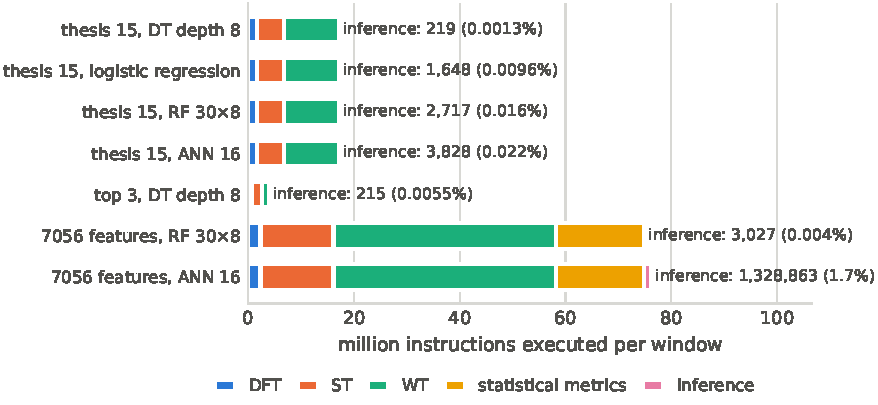
\includegraphics[width=0.95\linewidth]{fig-custo-etapas-en.pdf}
    \caption{Instructions executed per window, by extraction stage and in inference.}
    \label{fig:cost}
\end{figure}

For the reference set, the WT accounts for 60\% of the extraction instructions, the ST for 31\%, the DFT for 9\% and the statistical metrics for only 0.2\%. The weight of the WT comes from its undecimated form, in which each of up to eight levels filters all 2560 samples of each window. The ST, whose definition requires one inverse transform per harmonic, accounts for less than a third of the total thanks to the closed form of Equation~\eqref{eq:ts}, even though the THD is computed over all twenty harmonic orders. The implementation itself affects these numbers: removing the circular index handling from the interior of the WT filtering cut that stage's instructions by 32\%, with identical results.

As for memory, the flash of the reference set is dominated by the model in the RF's case, 113.2\,KB, while the extraction takes 4.0\,KB, CMSIS-DSP 5.8\,KB and the standard library 7.3\,KB. Static RAM, about 97\,KB for every family, is almost entirely the extraction's working buffers, namely each channel's transform coefficients, the ST's Gaussian tables and the WT's intermediate vectors. As a rough estimate, at one instruction per cycle at 168\,MHz, the extraction would take about 102\,ms, below the roughly 333\,ms of signal contained in the two windows.

\subsection{Effect of the feature set}
Table~\ref{tab:sets} shows the performance of each feature set with each model family, with the extraction instructions, and Figure~\ref{fig:f1-instructions} relates performance to computational cost for all configurations.

\begin{table}[htb]
  \centering
  \caption{Performance and extraction cost by feature set.}
  \label{tab:sets}
  \begin{tabular}{lrrrrr}
  \toprule
  \textbf{Set} & \textbf{LR} & \textbf{DT} & \textbf{RF} & \textbf{ANN} & \textbf{Instructions (millions)} \\
  \midrule
  Reference (15) & 0.680 & 0.741 & 0.781 & 0.689 & 17.2 \\
  Published (15) & 0.694 & 0.706 & 0.755 & 0.737 & 16.4 \\
  Top 10 & 0.639 & 0.699 & 0.776 & 0.669 & 16.0 \\
  Top 5 & 0.577 & 0.687 & 0.706 & 0.594 & 11.8 \\
  Top 3 & 0.467 & 0.572 & 0.577 & 0.488 & 3.9 \\
  Random (15), mean & 0.389 & 0.423 & 0.452 & 0.402 & 18.9 \\
  Random (15), maximum & 0.429 & 0.484 & 0.491 & 0.445 & 33.8 \\
  All (7056) & 0.653 & 0.780 & 0.754 & 0.632 & 74.8 \\
  \bottomrule
  \end{tabular}
  \note{macro-F1 on the 1645 test simulations. Extraction instructions per window; for the random sets, median and maximum over the ten draws.}
\end{table}

\begin{figure}[htb]
    \centering
    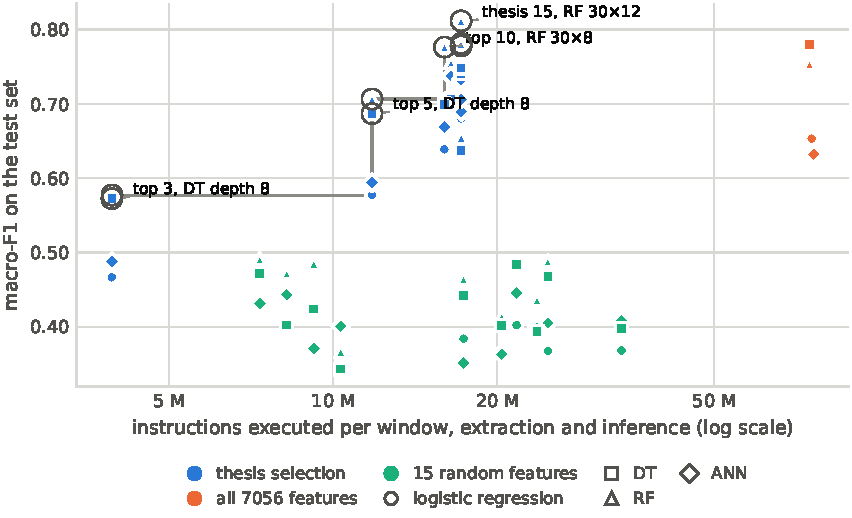
\includegraphics[width=0.95\linewidth]{fig-f1-instrucoes-en.pdf}
    \caption{Performance against instructions executed per window. Circled points form the front of configurations not beaten in both performance and cost at once.}
    \label{fig:f1-instructions}
\end{figure}

The reference set outperformed all ten random sets with every model family: even its worst result, 0.680 with the LR, beats the best random result, 0.491 with the RF. This is all the more relevant since the random sets take between 7.3 and 33.8 million instructions, with a median of 18.9 million, a cost comparable to the reference set's. Selection, therefore, does not reduce cost relative to an arbitrary set of the same size, but concentrates in it the information about the region.

Compared with the 7056 candidate features, the reference set needs 4.4 times fewer instructions and loses no performance. The RF reaches 0.781 with the reference set and 0.754 with all features, while the DT reaches 0.741 and 0.780, respectively, the only family where the full set is better. In addition, the full set needs 139 to 167\,KB of static RAM, which fits the microcontroller only by using the CCM, and 63 to 557\,KB of flash, depending on the model. When extracting all 7056 features, the statistical metrics account for 22\% of the instructions, against 0.2\% for the reference set.

The top features of the ranking show that cost can be reduced with a gradual loss of performance. The top ten reach 0.776 with the RF, practically the same as the full set of fifteen, with 16.0 million instructions, while the top five reach 0.706 with 11.8 million and the top three 0.577 with 3.9 million. The drop is sharpest for the top three because they skip most of the WT bands and ST voices. The published set performed close to the reference set, better with the LR and the ANN and worse with the DT and the RF, and this comparison is optimistic for the published set, which was selected with access to the test simulations.

Figure~\ref{fig:f1-flash} relates the same performance to flash. Unlike instructions, flash varies little with the feature set, staying between 18 and 22\,KB for every fifteen-feature set except with the RF. This is because the extraction code is the same for any set; only the table that configures it changes. Flash is thus set by the model, while feature selection sets the instructions executed and the RAM.

\begin{figure}[htb]
    \centering
    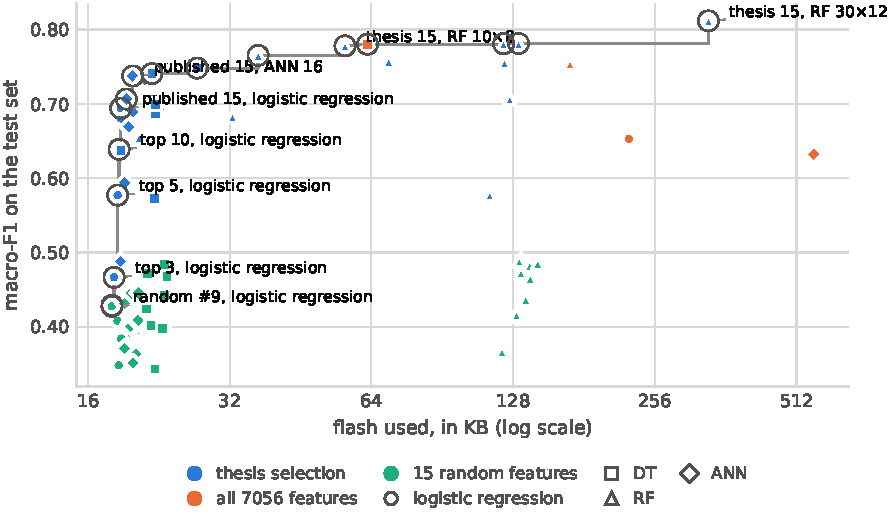
\includegraphics[width=0.95\linewidth]{fig-f1-flash-en.pdf}
    \caption{Performance against flash used.}
    \label{fig:f1-flash}
\end{figure}

\subsection{Model complexity and compiler optimization}
For the RF, going from 5 to 30 trees and from depth 4 to 12 raised macro-F1 from 0.655 to 0.812, the best result of the sweep, at the cost of 314\,KB of flash for the model, against 2.4\,KB for the smallest configuration. The gains, however, are not uniform. With ten trees of depth eight, the RF reaches 0.778 with 38\,KB, while thirty trees of the same depth add only 0.003 for 75\,KB more. For the DT, depth 4 gave 0.637 and depth 12 gave 0.748, close to the 0.741 of depth 8. For the ANN, eight, sixteen and thirty-two neurons gave 0.706, 0.689 and 0.733, with no monotonic trend. In every case, inference stayed below 6300 instructions, so model complexity essentially affects flash.

Speed optimization raised the extraction instructions by 3.2\%, from 17.17 to 17.71 million, cut the DT's inference instructions by 31\% and added 1.3 to 9.3\,KB of flash. More extraction instructions do not mean slower code, since this optimization level rearranges the code to save cycles in branches and memory accesses, an effect the functional simulator does not capture. This result illustrates the limitation discussed in Section~\ref{sec:measurement}.

\subsection{Fit to embedded devices}
The firmware of all 80 configurations fit the STM32F407, with at most 557\,KB of flash and 169\,KB of static RAM plus stack, the CCM being needed only for the 7056 features. No configuration would fit a microcontroller with 32\,KB of RAM, typical of the Cortex-M0+ class, since the smallest static RAM observed was 49\,KB.

One requirement, however, is not counted in these figures. In this work the raw windows live in flash as test data, but a real device would have to keep them in RAM as they are acquired. The two windows of the seven signals take 120 to 140\,KB in single precision, depending on the channels the set needs, which, added to the extraction's working buffers, exceeds the RAM of the microcontroller adopted.

% ----------------------------------------------------------
\section{Conclusion}

This work implemented the HIF region locator as C firmware for a simulated ARM Cortex-M4F microcontroller, from the feature set obtained by \citet{martins_tcc_en}, and measured the memory and computation it needs in 80 configurations. To keep the test set unseen, that work's selection chain was re-run on the training simulations only, and the resulting set was combined with logistic regression, a decision tree, a random forest and an artificial neural network.

The extraction was built on the CMSIS-DSP library, whose fast Fourier transform is limited to power-of-two lengths. The Stockwell transform, defined over a 2560-sample window, was obtained by decimation and by a closed form for the mean of each voice over each cycle, which avoids the inverse transforms, and the undecimated wavelet transform accumulates each cycle's RMS value during the filtering. In every configuration, the device's predictions agreed with the reference implementation's on at least 99\% of the test windows, and the features of the reference set were reproduced within tolerance on every window.

The results show that the locator's cost lies in the feature extraction, not in the model. For the reference set, extraction takes 17.17 million instructions per window, 60\% of them in the wavelet transform, while inference takes at most 0.02\% of the total. Feature selection cut this cost 4.4-fold compared with the 7056 candidate features with no loss of performance for the random forest, which reached a macro-F1 of 0.781, and outperformed every random set of the same size, whose cost is comparable. For the random forest, the top ten features of the ranking kept practically the same performance at a slightly lower cost. The choice of model, in turn, sets the flash, from 0.6\,KB for logistic regression to 314\,KB for the largest forest evaluated, which gave the best result, 0.812. The low computational cost argued in \citet{martins_tcc_en} thus holds on a microcontroller, with the caveat that the extraction, not the model, should be the focus of any optimization.

Some limitations must be considered. The simulator is functional, so executed instructions allow configurations to be compared but do not determine execution time, which depends on memory wait states and instruction latencies on the real device. In addition, the raw windows live in flash as test data, whereas a real device would have to store them in RAM, which exceeds the capacity of the microcontroller adopted. Finally, the signals come from simulations, the faulted phase is taken from metadata, as in \citet{martins_tcc_en}, and energy consumption was not measured.

\subsection*{Future work}
The results open several paths for continuing this work:
\begin{itemize}
    \item \textbf{Running on a real device:} running the same firmware on an STM32F4 board, reading the processor's cycle counter and measuring energy consumption, would turn the instructions measured here into time and energy, and check the real-time requirement.
    \item \textbf{Continuous signal acquisition:} replacing the stored windows by continuous acquisition, with analog-to-digital converters and direct memory transfer, and processing cycles as they arrive, would reduce the memory needed for the raw window, the main obstacle identified.
    \item \textbf{Reducing the extraction cost:} since extraction dominates the cost, optimizing the wavelet transform, shrinking the working buffers to the orders actually used and using fixed-point arithmetic could reduce instructions and RAM, as long as equivalence with the reference is preserved.
    \item \textbf{Comparison with quantized neural networks:} comparing with models run by TensorFlow Lite Micro \citep{david_tflm} in 8 bits would show the trade-off between precision and memory, even though inference is a small share of the total cost.
    \item \textbf{Including cost in feature selection:} the extraction cost of each feature, measured here, could become a criterion of the selection itself, favouring, among features of equivalent performance, those that are cheaper on the device.
\end{itemize}

\bibliographystyle{plainnat}
\bibliography{referencias,references-en}

\end{document}
